\subsection{Results}

The measurements of the characteristic curve of the detector are shown in Fig. \ref{fig::plateau}, together with the fit to the Geiger plateau, which will be explained later.
The middle of the plateau is at around \SI{740}{\volt}, so we will operate the system at this voltage for the rest of the experiment.

\begin{figure} [ht]
	\centering
	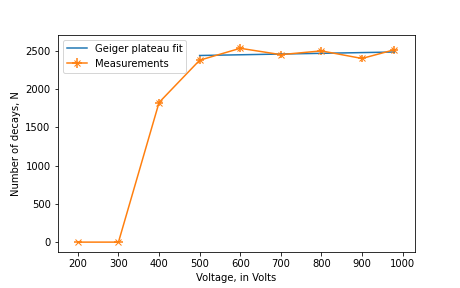
\includegraphics[width=400pt]{python/plateau.PNG}
	\caption{Number of counts plotted against voltage for duration of \SI{30}{\second}. Uncertainty only on voltage.}
	\label{fig::plateau}
\end{figure}

The uncertainty of the number of counts is described by the Poisson-distribution, therefore the uncertainty on any count is $\Delta N = \sqrt{N}$ \cite{manual}.
We measured an activity of $N = 7453 \pm  86$ decays, together with $N_{BG} = 50 \pm 7$ decays without the source.

As said, the distance is given as $d = 101 \pm \SI{0.5}{\milli\meter}$, and the diameter of the aperture we measured as $2*r = 18.05 \pm \SI{0.025}{\milli\meter}$.